\documentclass[border=2pt]{standalone}
\usepackage{tikz}
\usetikzlibrary{arrows.meta,chains,%
                    decorations.pathreplacing}
\usetikzlibrary{matrix,positioning,arrows.meta,arrows}

\tikzset{
mymat/.style={
  matrix of nodes,
  nodes in empty cells,
  text height=2.5ex,
  text depth=0.75ex,
  text width=3.25ex,
  align=center,
  column sep=-\pgflinewidth
  }
}
\tikzset{
  rows/.style 2 args={
    sub@rows/.style={row ##1 column #2/.style={nodes={rectangle,draw=black}}},
    sub@rows/.list={#1}
  },
  box/.style 2 args={
    sub@box/.style={rows={#1}{##1}},
    sub@box/.list={#2}
  }
}
\begin{document}

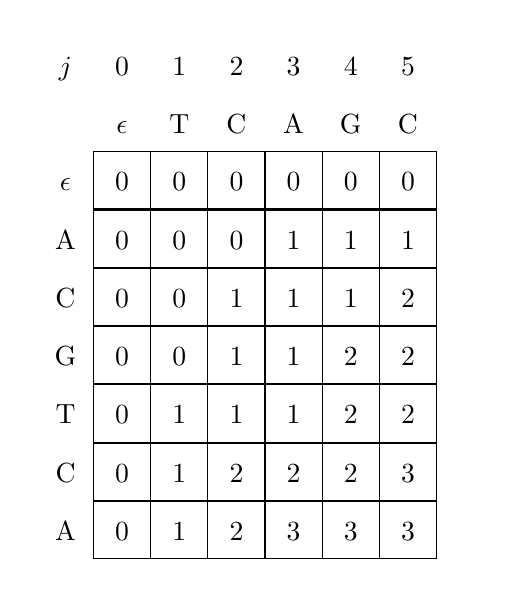
\begin{tikzpicture}[>=latex]
\matrix[mymat,anchor=west,
    box={3, 4, 5, 6, 7, 8, 9}{2, 3, 4, 5, 6, 7}]
at (0,0) 
(mat1)
{ 
  $j$ & 0 & 1 & 2 & 3 & 4 & 5 \\
  & $\epsilon$ 
        & T & C & A & G & C & \\
  $\epsilon$ 
    & 0 & 0 & 0 & 0 & 0 & 0 \\
  A & 0 & 0 & 0 & 1 & 1 & 1 \\
  C & 0 & 0 & 1 & 1 & 1 & 2 & \\
  G & 0 & 0 & 1 & 1 & 2 & 2 & \\
  T & 0 & 1 & 1 & 1 & 2 & 2 & \\
  C & 0 & 1 & 2 & 2 & 2 & 3 & \\
  A & 0 & 1 & 2 & 3 & 3 & 3 & \\
   };
\end{tikzpicture}

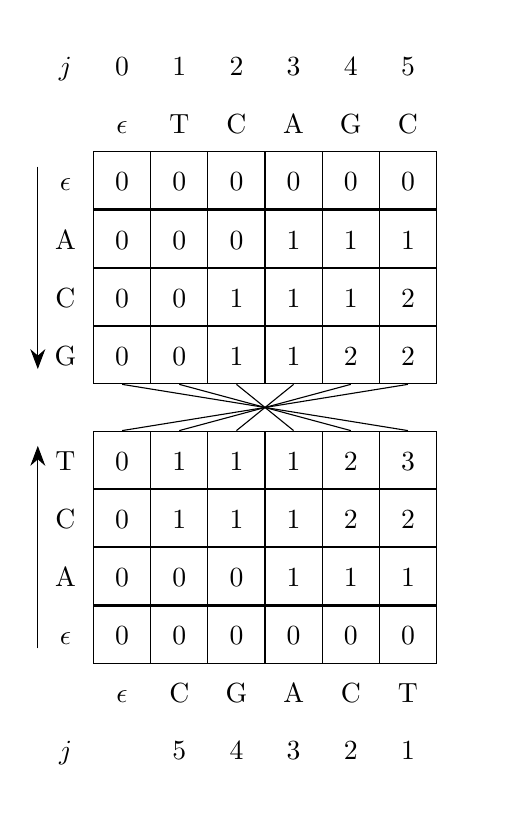
\begin{tikzpicture}[>=latex]
\matrix[mymat,anchor=west,
    box={3, 4, 5, 6}{2, 3, 4, 5, 6, 7}]
at (0,0) 
(mat1)
{ 
  $j$ & 0 & 1 & 2 & 3 & 4 & 5 \\
  & $\epsilon$ 
        & T & C & A & G & C & \\
  $\epsilon$ 
    & 0 & 0 & 0 & 0 & 0 & 0 \\
  A & 0 & 0 & 0 & 1 & 1 & 1 \\
  C & 0 & 0 & 1 & 1 & 1 & 2 & \\
  G & 0 & 0 & 1 & 1 & 2 & 2 & \\
   };
\matrix[mymat,anchor=west,
    box={1, 2, 3, 4}{2, 3, 4, 5, 6, 7}]
at (0,-5) 
(mat2)
{ 
  T & 0 & 1 & 1 & 1 & 2 & 3 \\
  C & 0 & 1 & 1 & 1 & 2 & 2 & \\
  A & 0 & 0 & 0 & 1 & 1 & 1 & \\
  $\epsilon$ 
    & 0 & 0 & 0 & 0 & 0 & 0 \\
  & $\epsilon$ 
        & C & G & A & C & T & \\
  $j$ & & 5 & 4 & 3 & 2 & 1 &  \\
   };

\begin{scope}
\coordinate(partA-start) at([xshift=-10pt,yshift=5pt]mat1-3-1.center);
\coordinate(partA-end) at([xshift=-10pt,yshift=-5pt]mat1-6-1.center);

\coordinate(partB-end) at([xshift=-10pt,yshift=5pt]mat2-1-1.center);
\coordinate(partB-start) at([xshift=-10pt,yshift=-5pt]mat2-4-1.center);

\draw[-{Stealth[scale=1.5]}] (partA-start) -- (partA-end);
\draw[-{Stealth[scale=1.5]}] (partB-start) -- (partB-end);
\end{scope}

\begin{scope}
\coordinate(start) at([xshift=0pt,yshift=0pt]mat1-6-2.south);
\coordinate(end) at([xshift=0pt,yshift=0pt]mat2-1-7.north);
\draw (start) -- (end);
\end{scope}

\begin{scope}
\coordinate(start) at([xshift=0pt,yshift=0pt]mat1-6-3.south);
\coordinate(end) at([xshift=0pt,yshift=0pt]mat2-1-6.north);
\draw (start) -- (end);
\end{scope}

\begin{scope}
\coordinate(start) at([xshift=0pt,yshift=0pt]mat1-6-4.south);
\coordinate(end) at([xshift=0pt,yshift=0pt]mat2-1-5.north);
\draw (start) -- (end);
\end{scope}

\begin{scope}
\coordinate(start) at([xshift=0pt,yshift=0pt]mat1-6-5.south);
\coordinate(end) at([xshift=0pt,yshift=0pt]mat2-1-4.north);
\draw (start) -- (end);
\end{scope}

\begin{scope}
\coordinate(start) at([xshift=0pt,yshift=0pt]mat1-6-6.south);
\coordinate(end) at([xshift=0pt,yshift=0pt]mat2-1-3.north);
\draw (start) -- (end);
\end{scope}

\begin{scope}
\coordinate(start) at([xshift=0pt,yshift=0pt]mat1-6-7.south);
\coordinate(end) at([xshift=0pt,yshift=0pt]mat2-1-2.north);
\draw (start) -- (end);
\end{scope}

\end{tikzpicture}

\end{document}